\subsection{Successioni di oggetti e morfismi}
\begin{frame}{Insiemi parzialmente ordinati come categorie}
    Sia $(X,\preceq)$ un insieme parzialmente ordinato.
    \pause

    È possibile considerarlo come una categoria $\mathcal{X}$ ponendo:
    \pause
    \begin{itemize}
        \item $\obj(\mathcal{X})=X$;
    \pause
        \item $\Hom(x,y)=
        \begin{cases}
            \emptyset & \text{se $x\npreceq y$} \\
            \{\iota^x_y\} & \text{se $x\preceq y$}
        \end{cases}$ per ogni $x,y\in\obj(\mathcal{X})$;
    \pause
        \item $\iota_y^x\cdot\iota_z^y=\iota_z^x$ se $x\preceq y\wedge y\preceq z$.
    \end{itemize}
\end{frame}

\begin{frame}{Insiemi parzialmente ordinati come categorie}
    
    \begin{example}[Topologia di uno spazio topologico]
        Sia $(X,\tau)$ uno spazio topologico. $(\tau,\subseteq)$ è parzialmente ordinato quindi può vedersi come una categoria i cui oggetti sono gli aperti e i cui morfismi sono le inclusioni.
    \end{example}
    \pause
        \begin{example}[Interi con diseguaglianze contrarie]
        Poniamo $n\preceq m\ssedef m\leq n$.
        \pause
        $(\mathbb{Z},\preceq)$ è totalmente ordinato, quindi parzialmente ordinato, e può vedersi come la categoria i cui oggetti sono gli interni e i cui morfismi sono le disuguaglianze contrarie:
        $$\cdots\longrightarrow\underset{n+1}{\bullet}\longrightarrow\underset{n}{\bullet}\longrightarrow\underset{n-1}{\bullet}\longrightarrow\cdots$$
    \end{example}
\end{frame}

\begin{frame}{Successioni di oggetti e morfismi}
    \begin{definition}[Successioni di oggetti e morfismi]
        Sia $\mathcal{C}$ una categoria.
        \pause

        Una \textbf{successione di oggetti e morfismi}, o \textbf{successione}, è un funtore covariante $S:\mathbb{Z}\rightarrow\mathcal{C}$:
        $$\cdots\longrightarrow A_{n+1}\xrightarrow{f_{n+1}}A_n\xrightarrow{f_n}A_{n-1}\longrightarrow\cdots$$
    \end{definition}

    \begin{block}{Osservazione}
        Analogamente, definiamo una \textbf{successione finita di oggetti e morfismi} di $\mathcal{C}$ come un funtore covariante
        $F:\mathrm{\mathbf{n+1}}\rightarrow\mathcal{C}$.
    \end{block}
\end{frame}

\begin{frame}{Successioni esatte}
    \begin{definition}[Successione esatta]
        Sia $A$ un anello commutativo.
        \pause

        Una successione finita o infinita di $A$-omomorfismi e $A$-moduli
        $$\cdots\longrightarrow M_{n+1}\xrightarrow{f_{n+1}}M_n\xrightarrow{f_n}M_{n-1}\longrightarrow\cdots$$
        si dice \textbf{successione esatta} se $\im f_{n+1}=\ker f_n$ per ogni $n$.
    \end{definition}
    \pause
    \begin{definition}[Successione esatta corta]
        Una \textbf{successione esatta corta} è una successione esatta della forma
        $$0\rightarrow A\xrightarrow{f}B\xrightarrow{g}C\rightarrow0$$
    \end{definition}
\end{frame}

\subsection{Categorie abeliane}
\begin{frame}{Categorie additive}
\begin{definition}[Categoria additiva]
    Una categoria $\mathcal{C}$ si dice \textbf{additiva} se
    \pause
    \begin{enumerate}[i.]
        \item $\Hom(A,B)$ è un gruppo abeliano per ogni $A,B\in\obj(C)$;
        \pause
        \item Vale la proprietà distribuitva sui morfismi: \pause dati
        $$X\xrightarrow{a}A\underset{g}{\overset{f}{\rightrightarrows}}B\xrightarrow{b}Y$$
        allora $(f+g)\cdot b=f\cdot b+g\cdot b$ e $a\cdot(f+g)=a\cdot f+a\cdot g$;
        \pause
        \item $\mathcal{C}$ ha un oggetto zero;
        \pause
        \item $\mathcal{C}$ ha prodotti finiti e coprodotti finiti.
    \end{enumerate}
\end{definition}
\end{frame}

\begin{frame}{Categorie additive}
    \begin{definition}[Funtore additivo]
        Siano $\mathcal{C}$ e $\mathcal{D}$ categorie additive.
        \pause

        Un funtore $F:\mathcal{C}\rightarrow\mathcal{D}$ si dice \textbf{additivo} se per ogni $A,B\in\obj(\mathcal{C})$ e per ogni $f,g\in\Hom(A,B)$ si ha
        $$F(f+g)=F(f)+G(g)$$
    \end{definition}
\end{frame}

\begin{frame}{Categorie abeliane}
    \begin{definition}[Categoria abeliana]
     Sia $\mathcal{C}$ una categoria. È abeliana se
    \pause
    \begin{enumerate}[i.]
        \item Ogni morfismo ha un kernel e un cokernel;
        \pause
        \item Ogni monomorfismo è un kernel e ogni epimorfismo è un cokernel.
    \end{enumerate}   
    \end{definition}
    \pause
    \begin{lemma}
        $\cat{Ab}$ è una categoria abeliana.
    \end{lemma}

\end{frame}

%%%%%%%%%%%%%%%%%%%%%%%%%%%%%%%%%%%%%%

\begin{frame}{Fasci di gruppi abeliani}
    \begin{definition}[Fascio di gruppi abeliani]
    Sia $(X,\tau)$ uno spazio topologico. 
    \pause
    Un \textbf{fascio di gruppi abeliani} su $X$ è un funtore controvariante
    $\mathcal{F}:\tau\rightarrow\mathrm{\mathbf{Ab}}$
    tale che:
    \pause
    \begin{itemize}
        \item Ad ogni aperto $A$ associa un gruppo abeliano $\mathcal{F}(A)$;
        \pause
        \item A $\iota_B^A$ associa $\mathcal{F}(\iota_B^A)=\rho^B_{|A}\in \Hom(\mathcal{F}(B),\mathcal{F}(A))$;
        \pause
        \item \textbf{Unicità}: Per ogni $A\in\tau$ e suo ricoprimento aperto $(A_i)_{i\in I}$, se per ogni $g,h\in\mathcal{F}(A)$ si ha $\rho^A_{|A_i}(g)=\rho^A_{|A_i}(h)\ \forall\ i$, allora $g=h$;
        \pause
        \item \textbf{Incollamento}: $\forall\ A\in\tau$ e suo ricoprimento aperto $(A_i)_{i\in I}$, se comunque presi $\sigma_i\in\mathcal{F}(A_i)$, si ha $\rho^A_{|A_i\cap A_j}(\sigma_i)=\rho^A_{|A_i\cap A_j}(\sigma_j)$ per ogni $i$ e $j$, allora $\exists!\sigma\in\mathcal{F}(A)$ tale che $\rho^A_{U_i}(\sigma)=\sigma_i\ \forall\ i$.
    \end{itemize}
    \end{definition}
\end{frame}



\begin{frame}{La categoria dei fasci di gruppi abeliani}
    I fasci di gruppi abeliani costituiscono una categoria. In particolare, dato uno spazio topologico $(X,\tau)$:
    \pause
    \begin{definition}[Categoria dei fasci di gruppi abeliani]
        Definaimo $\mathrm{\mathbf{Sh}}(X,\mathrm{\mathbf{Ab}})$ come la categoria tale che:
        \pause
        \begin{itemize}
            \item $\obj(\cat{Sh}(X,\cat{Ab}))$ è costituito dai fasci $\tau\rightarrow\cat{Ab}$;
            \pause
            \item $\Hom(\mathcal{F},\mathcal{G})$ è costutito dalle trasformazioni naturali $\mathcal{F}\rightarrow\mathcal{G}$.
        \end{itemize}
    \end{definition}
    \pause
    \begin{lemma}
        $\cat{Sh}(X,\cat{Ab})$ è una categoria abeliana.
    \end{lemma}
\end{frame}


\begin{frame}{Risoluzioni iniettive di fasci}
\begin{definition}[Fasci iniettivi]
Sia $\mathcal{F}$ un fascio di gruppi abeliani.
\pause

$\mathcal{F}$ è \textbf{iniettivo} se per ogni monomorfismo $g:\mathcal{G}\rightarrowtail\mathcal{H}$ e per ogni morfismo $f:\mathcal{G}\rightarrow\mathcal{F}$, esiste $h:\mathcal{H}\rightarrow\mathcal{F}$ che rende commutativo il seguente diagramma:
\[
        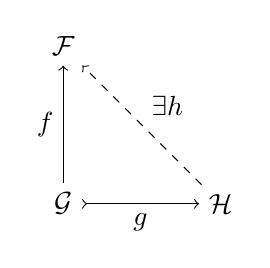
\begin{tikzpicture}[->, node distance=2cm]
        \node (E) {$\mathcal{F}$};
        \node (A) [below of=E] {$\mathcal{G}$};
        \node (B) [right of=A] {$\mathcal{H}$};

        \draw (A) -- (E) node[midway, left] {$f$};
        \draw[>->] (A) -- (B) node[midway, below] {$g$};
        \draw[dashed] (B) -- (E) node[midway, above right] {$\exists h$};

        \end{tikzpicture}
\]
\end{definition}    
\end{frame}

\begin{frame}{Risoluzioni iniettive di fasci}
    \begin{definition}[Risoluzione iniettiva di fasci]
        Sia $\mathcal{F}$ un fascio di gruppi abeliani.
        \pause
        Una \textbf{risoluzone iniettiva di $\mathcal{F}$} è una successione esatta di fasci
        $$\mathrm{\mathbf{E}}=0\longrightarrow\mathcal{F}\longrightarrow\mathcal{G}^0\longrightarrow\mathcal{G}^1\longrightarrow\mathcal{G}^2\longrightarrow\cdots$$
        con $\mathcal{G}^n$ iniettivo per ogni $n\in\mathbb{N}_0$.
    \end{definition}
    \pause
    \begin{definition}[Risoluzione inieittiva di fasci troncata]
        Alla risoluzione iniettiva  di fasci $\mathrm{\mathbf{E}}$ è possibile associare il complesso
        $$\mathrm{\mathbf{E}}^{\mathcal{F}}=0\longrightarrow\mathcal{G}^0\longrightarrow\mathcal{G}^1\longrightarrow\mathcal{G}^2\longrightarrow\cdots$$
        detto \textbf{risoluzione iniettiva troncata}.
    \end{definition}
\end{frame}

\subsection{Fasci}
%Riassumiamo l'argomento di Nino:



\begin{frame}{Fasci di gruppi abeliani}
    \begin{definition}[Funtore delle sezioni globali]
        Il \textbf{funtore delle sezioni globali} è il funtore covariante additivo
        $$\Gamma:\mathrm{\mathbf{Sh}}(X, \mathrm{\mathbf{Ab}})\rightarrow\mathrm{\mathbf{Ab}}$$
        tale che
        \pause
        \begin{itemize}
            \item Ad ogni fascio $\mathcal{F}$ su $X$, associa $\mathcal{F}(X)$;
        \pause
            \item Al morfismo di fasci $\varphi:\mathcal{F}\rightarrow\mathcal{G}$ associa $\varphi_X:\mathcal{F}(X)\rightarrow\mathcal{G}(X)$.
        \end{itemize}
    \end{definition}
\end{frame}




\section{Coomologia di fasci}

\begin{frame}
    Si fissi uno spazio topologico $(X,\tau)$.
    \pause
    \begin{definition}[Coomologia di fasci]
        \pause
        Siano $\mathcal{F}$ un fascio di gruppi abeliani su $X$ e $$\mathrm{\mathbf{E}}=0\longrightarrow\mathcal{F}\xrightarrow{\eta}\mathcal{G}^0\xrightarrow{d^0}\mathcal{G}^1\xrightarrow{d^1}\mathcal{G}^2\longrightarrow\cdots$$
        una risoluzione iniettiva di $\mathcal{F}$.
        \pause
        $$H^q(\mathcal{F})\coloneq H^q\left(\Gamma{\mathrm{\mathbf{E}}}^\mathcal{F}\right)=\frac{\ker\left(\Gamma(d^q):\Gamma(\mathcal{G}^q)\rightarrow\Gamma({\mathcal{G}}^{q+1})\right)}{\im\left(\Gamma(d^{q-1}):\Gamma(\mathcal{G}^{q-1})\rightarrow\Gamma({\mathcal{G}}^{q})\right)}$$
        \pause
        dove $\mathrm{\mathbf{E}}^\mathcal{F}$  è la risoluzione troncata associata ad $\mathrm{\mathbf{E}}$ e $\Gamma$ è il funtore delle sezioni globali.
    \end{definition}
\end{frame}